%% Overleaf			
%% Software Manual and Technical Document Template	
%% 									
%% This provides an example of a software manual created in Overleaf.

\documentclass{ol-softwaremanual}

% Packages used in this example
\usepackage{graphicx}  % for including images
\usepackage{microtype} % for typographical enhancements
\usepackage{minted}    % for code listings
\usepackage{amsmath}   % for equations and mathematics
\usepackage{mathrsfs}  % for \mathscr (script H interaction coefficient)
\setminted{style=friendly,fontsize=\small}
\renewcommand{\listoflistingscaption}{List of Code Listings}
\usepackage{hyperref}  % for hyperlinks
\usepackage[a4paper,top=4.2cm,bottom=4.2cm,left=2.0cm,right=2.0cm]{geometry} % for setting page size and margins
\usepackage{booktabs,tabularx}
\usepackage{xltabular}
\usepackage[input-decimal-markers=.]{siunitx}
\usepackage{lipsum}
\usepackage{lscape}
\usepackage{graphicx}
\usepackage{subcaption}
\usepackage[colorinlistoftodos]{todonotes}
\usepackage{fancyhdr}
\usepackage{listings}
\usepackage{xcolor}
\usepackage[backend=biber,style=ieee,sorting=ynt]{biblatex}

\definecolor{codegreen}{rgb}{0,0.6,0}
\definecolor{codegray}{rgb}{0.5,0.5,0.5}
\definecolor{codepurple}{rgb}{0.58,0,0.82}
\definecolor{backcolour}{rgb}{0.95,0.95,0.92}

\lstdefinestyle{mystyle}{
    backgroundcolor=\color{backcolour},   
    commentstyle=\color{codegreen},
    keywordstyle=\color{magenta},
    numberstyle=\tiny\color{codegray},
    stringstyle=\color{codepurple},
    basicstyle=\ttfamily\footnotesize,
    breakatwhitespace=false,         
    breaklines=true,                 
    captionpos=b,                    
    keepspaces=true,                 
    numbers=left,                    
    numbersep=5pt,                  
    showspaces=false,                
    showstringspaces=false,
    showtabs=false,                  
    tabsize=2
}
\addbibresource{CFDwavemaker.bib}
\lstset{style=mystyle}

% Custom macros used in this example document
\newcommand{\doclink}[2]{\href{#1}{#2}\footnote{\url{#1}}}
\newcommand{\cs}[1]{\texttt{\textbackslash #1}}

% Frontmatter data; appears on title page
\title{CFDwavemaker \\User Manual (DRAFT)}
\version{3.0.1}
\author{Øystein Lande}
%\softwarelogo{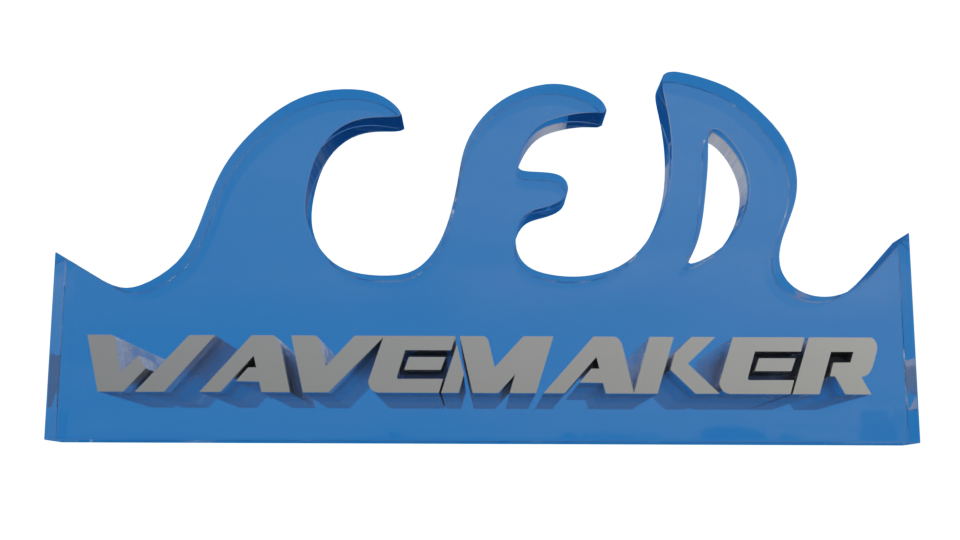
\includegraphics[width=8cm]{logo.png}}

\begin{document}

\maketitle

\tableofcontents
%\listoflistings
\newpage

\section{Introduction}
\subsection{Purpose}
CFDwavemaker is a C++ library developed with the purpose of providing wave kinematics input to CFD codes. Kinematics may either be generated at the boundary (similar to a traditional wave maker) or used to initialize the entire domain before startup of the simulation (or both), as illustrated in the figure below. What distinguishes CFDwavemaker from other similar codes is its capability of generating irregular short crested waves with several hundreds of frequency components using second order potential wave theory in a numerically efficient way.
\begin{figure}[htbp]
    \centering
    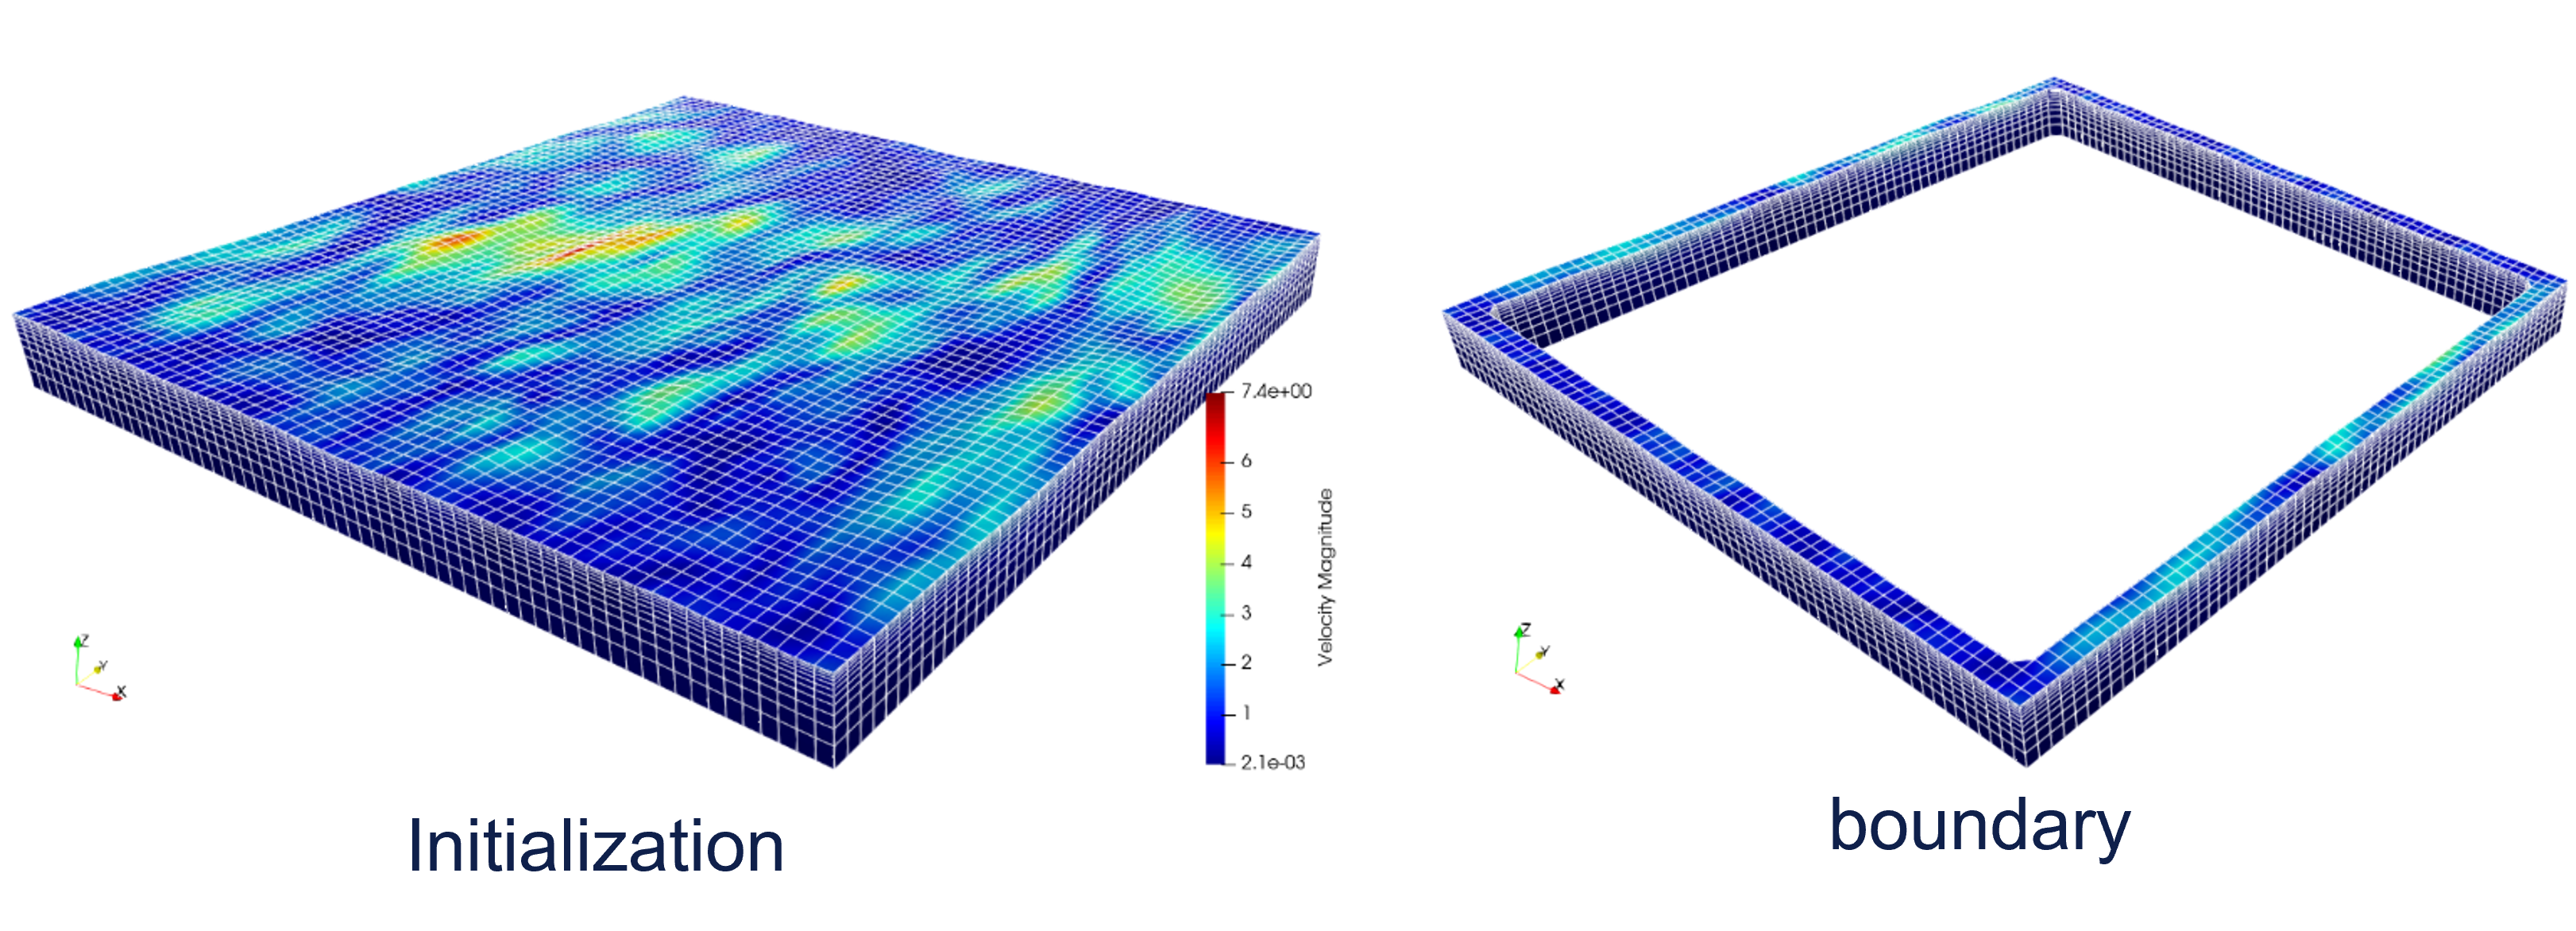
\includegraphics[width=16cm]{cfdwavemaker_purpose.png}
    \caption{Kinematics examples needed for initialization of CFDdomain (left) or during runtime at the boundaries (right)}
    \label{fig:lsgrid}
\end{figure}

The library have been successfully linked to a number of CFD solver, such as the Basilisk Library, OpenFOAM, ComFLOW, StarCCM+. It can be accessed and linked to any programming language which support C binding (Python, C/C++, Fortran, and more.)
\subsection{Reference}
The code is open source and free to use by anyone. If you find the code useful and decide to used it in projects or publications, make sure spread the word by referencing to this paper
\begin{lstlisting}[numbers=none]
@inproceedings{landeCFDwavemaker,
   title={CFDWAVEMAKER: An open-source library for efficient generation of higher order wave kinematics},
   author={Lande, Oystein and Helmers, Jens Bloch},
   booktitle={International Conference on Offshore Mechanics and Arctic Engineering},
   volume={57656},
   pages={V03AT02A029},
   year={2022},
   organization={American Society of Mechanical Engineers}
}
\end{lstlisting}

\section{Installation}
\subsection{Operative system and requirements}
CFDwavemaker
\subsection{Compile from Source}
Start by cloning the \doclink{https://github.com/oystelan/CFDwavemaker}{git repository} into a suitable location on you computer.
\begin{lstlisting}[numbers=none]
git clone git@github.com:oystelan/CFDwavemaker.git
\end{lstlisting}
open a terminal and navigate to the location of the CFDwavemaker folder. a Makefile is provided for quick building. CFDwavemaker can be built in three different versions:
\begin{itemize}
    \item \textbf{default}: contains core kinematics library + the SWD library extension.
    \item \textbf{basic}:The core kinematics library, excluding SWD. SWD requires a fairly new version of gcc or intel compiler on windows. Therefore it can sometimes be useful to exclude SWD from the build if you dont plan on using it.
    \item \textbf{all}: Complete build, linking core library, swd and the vtk library into one dynamic library. This does however require a bit of preparation, like builting the vtk library upfront, and modifying the make script accordingly to be in line with the version of vtk you have built. Dont attempt this if your not experienced with compiling.
    \item \textbf{mpi}: The core kinematics library built with MPI support. This is intended for large domains where the LSgrid second-order kinematics are expensive to compute: when built with MPI the grid update is distributed across ranks (each rank computes a block of the domain, and the result is shared with an \texttt{MPI\_Allgatherv}), rather than every rank redundantly computing the whole domain. See Section~\ref{sec:mpi} for details.
\end{itemize}
So, to build the basic version, you execute the following two commands:
\begin{lstlisting}[numbers=none]
make clean
make basic
\end{lstlisting}
or to build the complete library (including swd and vtk support), you do:
\begin{lstlisting}[numbers=none]
make clean
make all
\end{lstlisting}
and to build the MPI-enabled library:
\begin{lstlisting}[numbers=none]
make mpi
\end{lstlisting}
(the \texttt{mpi} target cleans and rebuilds automatically, since it uses different compiler flags than the other targets).

If the target is omitted, the default version is built. If everything went according to plan, the resulting static and dynamic link library should now have turned up in the folder ../build/linux64/* Thats it, in terms of building the library. Now its time to link the library to your software of choice.

\subsection{Dependencies}
So why did i choose to build the basic version? The answer is, for the default version (containing the =swd extension) and for the all package which links to vtk, there are some dependencies you need which does not by default ship with the compiler.

For the default version of CFDwavemaker, the only additional dependency is fftw3. This is easily installed on a debian based system with the following command:

\subsection{From binary}
The latest build for Linux (normally latest release of Ubuntu) is possible to download from \doclink{https://github.com/oystelan/CFDwavemaker}{the CFDwavemaker repository}.


\section{Interpolation Schemes}
Grid interpolation schemes are essential in order to speed up initialization of CFD domains when using computationally expensive wave theories such as second order irregular wave theory and HOSM. The cell resolution in a CFD simulation where the kinematics components are required may be fare greater than what is needed to define the kinematics of the wave field with adequate accuracy. Using interpolation in time and space will thus save lots of computation (and time). In addition, defining kinematics on a grid rather than doing point by point randomly, simplifies parallelization.

\textbf{Note:}Grid interpolation is currently only supported for use with SWD and second order irregular wave theory. For linear irregular waves or regular wave theories the use of grid interpolation will not result in a significant gain in performance.
\subsection{Lagrangian Stretch grid (LSgrid)}
The following statements can be said to be true for the kinematics vector field underneath an irregular sea surface:
\begin{itemize}
    \item The velocity profiles are exponential
    \item The largest velocities occurring at the surface
    \item The largest spatial velocity gradients occur near the free surface
    \item Wave kinematics above the free surface is irrelevant.
\end{itemize}
The last statement might be obvious, but is what you will end up storing if your interpolation mesh is static. At the same time you will need to extrapolate the kinematics above the free surface to avoid loosing energy when the mesh is used for interpolation by the CFD solver. The best alternative is thus to have a mesh that moves with the free surface and that has a high density of cells close to the surface, an coarser for increasing water depths. The Lagrangian-Stretched grid (in short LSgrid) is just that! A mesh structure optimized for storage of wave kinematics data and that allows for the use of simple interpolation techniques.
LSgrid uses sigma transforms in combination with a stretching factor, giving high resolution in z direction at the surface, and lower at depth. The upper layer of the LSgrid will always be at the free surface, and the bottom layer will always be at the sea bed, such that all points of the mesh covers the fluid only. An example snapshot of such a grid is shown in the figure below. This provides a very efficient way of describing the velocity profile underneath the sea surface accurately with a minimum number of points. The time interpolation is linear. To specify the use of a Lagrangian stretched grid interpolation scheme, the keyword \textbf{[lsgrid]} is used.
\begin{figure}[htbp]
    \centering
    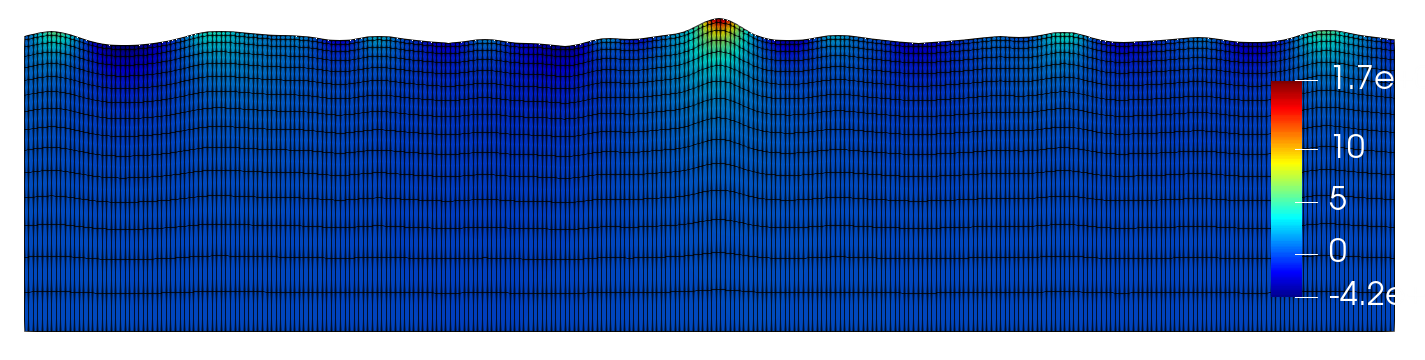
\includegraphics[width=16cm]{lsgrid2.png}
    \caption{Lagrangian stretch grid using $\sigma$-coordinates}
    \label{fig:lsgrid}
\end{figure}


\subsection{Cubic Spline 4D interpolation}


\subsection{Distributed grid computation with MPI}\label{sec:mpi}
Generating the second-order kinematics on the LSgrid is the most expensive part of a large simulation: every grid point requires a sum over all (possibly several hundred) frequency-pair interactions. With shared-memory parallelism (OpenMP) this is already spread over the cores of a single node. For very large domains run on an MPI-parallel CFD solver, however, \emph{every} MPI rank would by default recompute the \emph{entire} grid, which is wasteful. The MPI build removes this redundancy.

When CFDwavemaker is compiled with the \textbf{mpi} target (see the build instructions in the Installation section), the LSgrid computation is \emph{distributed}: on each grid update every rank computes only a block of the domain (a contiguous range of grid columns), and the blocks are then shared among all ranks with a single collective \texttt{MPI\_Allgatherv}. Afterwards every rank holds the complete, identical grid, so the interpolation (and everything downstream) is unchanged --- only the cost of \emph{building} the grid is divided among the ranks. The column partition is \emph{work-balanced} by the number of active cells per column, so an \texttt{ignore\_subdomain} mask (which makes some columns cheap) does not leave ranks idle.

A few things are required of the host CFD solver when using the MPI build:
\begin{itemize}
    \item \textbf{The host owns MPI.} CFDwavemaker never calls \texttt{MPI\_Init} or \texttt{MPI\_Finalize}; it only uses the MPI context that the CFD solver has already set up.
    \item \textbf{Collective update.} The grid update is a collective operation, so \emph{all} ranks in the communicator must reach it together. In practice this means every rank must call \texttt{wave\_force\_update(t)} once per time step, with the same \texttt{t}. This function is the designated synchronisation point; the ordinary velocity/elevation queries never trigger a grid update on their own.
    \item \textbf{Communicator.} By default the world communicator (\texttt{MPI\_COMM\_WORLD}) is used. If your solver runs CFDwavemaker on a sub-communicator, pass it with \texttt{wave\_set\_mpi\_comm(fortran\_comm)} (a Fortran integer communicator handle; use \texttt{MPI\_Comm\_c2f} in C) \emph{before} calling \texttt{wave\_Initialize()}.
    \item \textbf{No OpenMP.} The MPI build does not use OpenMP (it is one or the other); parallelism comes entirely from the MPI ranks.
\end{itemize}
Note that this distributes \emph{computation}, not memory: every rank still stores the full grid, exactly as in the shared-memory build. The MPI build is therefore aimed at cases where the second-order grid generation dominates the run time, not at reducing per-rank memory.

\section{Input file reference}

\subsection{[wave type]}
CFDwavemaker currently support the following wave theories. Which branch of wave theory to used is controlled by the keyword \textbf{[wave type]}
\begin{enumerate}
    \item \textbf{irregular} - irregular wave theory (linear or second order)
    \item \textbf{regular} - Stokes regular wave theory (up to 5th order)
    \item \textbf{piston} - Wave maker theory
    \item \textbf{swd} -  Spectral-Wave-Data file (swd)
    \item \textbf{vtk} - VTK library is another external library which is supported by most CFD programs. By building and linking this with CFDwavemaker, kinematics can be imported from any program capable of writing vtk files.
    \item \textbf{slope} - Initialise with water at rest with a given slope
\end{enumerate}

To chose one of the above use the following code word
\begin{lstlisting}[]
[wave type]
# This is a comment
irregular
\end{lstlisting}
where any lines starting with \# are regarded as comments in the input file and will be ignored during execution.

\subsection{[general input data]}
Some data are mandatory for all wave types. These parameters are specified under the keyword \textbf{[general input data]}.

\begin{table}[!htbp]
\renewcommand{\arraystretch}{1.5} 
\begin{tabularx}{\textwidth}{@{}lXl@{}}
\toprule
\multicolumn{1}{l}{Variable}&\multicolumn{1}{l}{Description}&\multicolumn{1}{r}{Default}\\
\midrule
depth&Water depth used to generate wave height & No\\
mtheta&(mean) wave direction. In case of long-crested unidirectional waves, this input prepresents the wave direction, while for short-crested waves, this represents the mean wave direction. Value is given in degrees where a value of 0 corresponds to wave propagating along the x-axis in the positive direction.&Yes(0)\\
swl&Still water level. default value = 0.&No\\
normalize&Normalize the wave by dividing the spectral values by the spectral 0th moment. This is useful to produce focused irregular waves. Default value = 0 (False)&No\\
gravity&gravity, which by default is set to 9.81 m/s\textsuperscript{2}&yes(9.81)\\
amplify&Gain factor applied to all wave amplitudes. Useful for scaling the wave field up or down.&yes(1.0)\\
rho&water density, which by default is set to 1025 kg/m\textsuperscript{3}&yes(1025)\\
nhpres\_include\_kinetic&Controls the form of the nonhydrostatic pressure returned by \texttt{wave\_nhPres}. When \texttt{false} (default): linearized form $p_{nh} = -\rho(\partial\phi/\partial t + g\eta)$, suitable for use as a pressure boundary condition in non-hydrostatic CFD solvers (where the kinetic energy is captured by the convective terms in the solver's momentum equations). When \texttt{true}: full Bernoulli form $p_{nh} = -\rho(\partial\phi/\partial t + \tfrac{1}{2}|\mathbf{u}|^2 + g\eta)$, matching the pressure field that a fully-resolved CFD code would compute internally. Currently active for \texttt{wave\_nhPres} with SWD (\texttt{[wave type] = swd}).&yes(false)\\
%scale&Froude scaling factor, used to scale output. & yes(1.0) \\
\bottomrule
\end{tabularx}
\end{table}
Finally, an example:
\begin{lstlisting}[]
[general input data]
depth  1.2
mtheta  0.0000
swl  0.
normalize  0
amplify  1.
%scale 1.0
\end{lstlisting}
%\subsubsection{Note on Froude scaling}
%Froude scaling of the output kinematics can sometime be useful. To be completely clear about the implementation, a list of statements are given
%\begin{itemize}
%    \item A scale factor $S_F$ less than 1.0, implies shrinking the domain which you extract kinematics. Scale factor $S_F$ greater than 1.0, implies enlarging.
%    \item There are different scaling laws. We stick to Froude scaling law for now.
%    \item both time and velocity scale with $S_F=\sqrt{scale}$.
%    \item Lengths and pressure scales with $S_F=scale$
%    \item $\eta_{scaled}(S_Fx,S_Fy,\sqrt{S_F}t) = S_F \eta(x,y,t)$$\
%\end{itemize}

\subsection{[wave reference point]}
A reference point in time and space for the wave specification is needed. This is specified using the tag \textbf{[wave reference point]}, as shown in the example given below. time is given in seconds, position x and y are given in meters. Specifying the \textbf{[wave reference point]} is optional. If this is not given, default values will be assumed.

\begin{table}[!htbp]
\renewcommand{\arraystretch}{1.5} 
\begin{tabularx}{\textwidth}{@{}lXl@{}}
\toprule
\multicolumn{1}{l}{Variable}&\multicolumn{1}{l}{Description}&\multicolumn{1}{l}{Default}\\
\midrule
time& reference point in time. & yes(0.)\\
x&reference point in space, x-axis.&Yes(0.)\\
y&reference point in space, y-coordinate.&Yes(0.)\\
\bottomrule
\end{tabularx}
\end{table}

\begin{lstlisting}[]
[wave reference point]
# for focused waves this will correspond to the focus point in time and space
time  15.0
x  3.5
y  0.0
\end{lstlisting}

\subsection{[ramps]}
Ramps can sometimes be useful to avoid transient behaviour for example in at startup, or when specifying wave kinematics in corners of a domain. Ramps are specified in time and space (x and y plane only) by calling the keyword [ramps] followed by the ramp input. The ramp may be omitted all together, in which case no ramp of any kind is used.

\begin{table}[!htbp]
\renewcommand{\arraystretch}{1.5} 
\begin{tabularx}{\textwidth}{@{}lXl@{}}
\toprule
\multicolumn{1}{l}{Variable}&\multicolumn{1}{l}{Description}&\multicolumn{1}{l}{Default}\\
\midrule
time\_rampup&Adds a time rampup. Two values follow: the starttime and end time of the ramp. The function starts at a value of 0.0 at t <= starttime, and increases linearly towards a value of 1.0 at t >= endtime. Omit the keyword to disable.& disabled\\
time\_rampdown&Adds a time rampdown. Two values follow: the starttime and end time of the ramp. The function starts with a value of 1.0 at time <= starttime, and linearly goes towards 0.0 at endtime. Omit the keyword to disable.&disabled\\
x\_rampup&Adds a rampup in x-direction. Two values follow: the start position and end position of the ramp. The function starts at a value of 0.0 at x <= startpos, and increases linearly towards a value of 1.0 at x >= endpos. Omit the keyword to disable.&disabled\\
x\_rampdown&Adds a rampdown in x-direction. Two values follow: the start position and end position of the ramp. The function starts with a value of 1.0 at x <= startpos, and linearly goes towards 0.0 at endpos. Omit the keyword to disable.&disabled\\
y\_rampup&same description as x\_rampup, only for y-direction&disabled\\
y\_rampdown&same description as x\_rampdown, only for y-direction&disabled\\
\bottomrule
\end{tabularx}
\end{table}
\begin{lstlisting}[]
[ramps]
# rampname starttime endtime
time_rampup  0.0000  3.0
# rampname startpos endpos
x_rampup  -11.0000  -10.0
x_rampdown  11.0000  12.0
\end{lstlisting}




\subsection{[wave input irregular]}
\begin{table}[!htbp]
\renewcommand{\arraystretch}{1.5} 
\begin{tabularx}{\textwidth}{@{}lXl@{}}
\toprule
\multicolumn{1}{l}{Variable}&\multicolumn{1}{l}{Description}&\multicolumn{1}{l}{Default}\\
\midrule
kinematics\_surf\_extrap& Switch between first order (linear and second order irregular wave kinematics. The default is second-order theory (2), with Taylor expansion of the kinematics profile above the SWL, consistent to second order. Generally, it is recommended to use second-order kinematics whenever the steepness is $ak > 0.1$.
You may occasionally want to use linear wave theory. In such an event, you should set this parameter to 1. If linear wave kinematics is specified, kinematics for z > 0 will be equal to the kinematics at z=0.
If you wish to use exponential extrapolation instead of a constant, you can set the parameter to 0. & 2 \\

vertical\_theory& Vertical structure used for the second-order kinematics. The default (\texttt{sharma}, or omitting the keyword) uses the conventional Sharma \& Dean profile with Taylor extrapolation of the kinematics above the SWL. Setting \texttt{vertical\_theory smit} selects the boundary-fitted $s$-coordinate (``sigma'') formulation of Smit et al.\ (2017): the vertical profile follows the instantaneous free surface rather than being extrapolated, which is better behaved for steep crests. \textbf{Note: the \texttt{smit} option is EXPERIMENTAL / in development} --- the self-interaction (diagonal) terms are validated against exact Stokes theory, but the off-diagonal second-order interactions are still being verified, so it is not yet recommended for production use. See Section~\ref{app:eq9_correction} for the implementation status and the corrections applied to the published equations.& sharma \\

bandwidth&control the bandwidth of which frequencies that are allowed to interact in the second-order sum and difference terms. For wide band spectra this is recommended. default value is “off”, which implies that all frequencies are allowed to interact in second-order terms. Alternatively bandwidth=auto can be used and CFDwavemaker will approximate a reasonable bandwidth for you from the spectral moments, i.e bandwidth``=0.7*m0/m1. The third alternative is to specify a value given in rad/s.&Yes(auto)\\

cutoff&High-frequency cut-off for the second-order sum and difference interactions. Frequencies above this value will not contribute to second-order terms. Units in rad/s.&Yes(100000)\\


individual\_ramp & If set to True, an additional three columns must be specified when giving the frequency component below. The three columns are ramp length, ramp start-up time, and duration. This gives full flexibility in switching on and off of single-frequency components at specific times. By default, all frequency components are turned on and will not be ramped in unless specified with this option & False \\

nfreq&number of frequency components to read from input file. A list of frequency component data should follow, where the number of entries (lines) must correspond to the number of components specified with this parameter. For each component, the following data should be given on a single line, separate by space: 1. frequency: given in rad/s. 2. amplitude: given in metres. 3. wave number: wave number associated with frequency (specified in rad/m). 4. phase: Random phase, value between 0 and 2*PI (specified in radians). 5. theta: (only specified if ``ndir``= 0) direction of frequency component (specified in radians).&no\\

ndir&number of directional components and the associated wave spreading, to read from input file. The directional components should follow directly after the list of frequency component data. ndir may be set to zero, in which case the library will look for an additional fifth column in the list of frequency component data, specifying the direction of each single frequency component.&no\\
\bottomrule
\end{tabularx}
\end{table}
Immediately following the specification of of the parameters \textbf{nfreq} and \textbf{ndir}, follows a list of irregular wave components. The length of the list must naturally match the number of frequency and directional components specified. Here are a couple of examples.

Example1:
\begin{lstlisting}[]
individual_ramp True
nfreq 5
ndir 0
# OMEGA [rad/s]    A[m]       K[rad/m]        Phase[rad]    theta[rad]  rampup_length[sec] ramp_startup_time[sec] duration[sec]
0.80684460     0.09098686     0.06636591    22.09105101    -0.51238946  1.0                2.0                    15.0
0.57527858     0.08989138     0.03410555    -8.15520380    -1.01219701  1.0                1.8                    15.0
0.59315305     0.20143761     0.03615181    -8.35009702    -0.92729522  1.0                1.6                    15.0
0.71493207     0.09704876     0.05213889    11.00239563    -0.58800260  1.0                1.4                    15.0
0.73560378     0.15043259     0.05518335    14.76881712    -0.55165498  1.0                1.2                    15.0
\end{lstlisting}

Example2:
Linear wave theory specified in this case
\begin{lstlisting}[]
kinematics_surf_extrap 1
nfreq 4
ndir 19
# OMEGA [rad/s] A [m]     K          Phase [rad]
    5.2033     0.0369     2.7670     0.0000
    5.3014     0.0356     2.8708     0.0000
    5.3996     0.0343     2.9767     0.0000
    5.4978     0.0331     3.0849     0.0000
# DIRS [rad]      Density
    -0.7854       0.042843
     -0.69813     0.045853
     -0.61087     0.048652
      -0.5236     0.051192
     -0.43633     0.053426
     -0.34907     0.055313
      -0.2618     0.056819
     -0.17453     0.057916
    -0.087266     0.058583
            0     0.058806
     0.087266     0.058583
      0.17453     0.057916
       0.2618     0.056819
      0.34907     0.055313
      0.43633     0.053426
       0.5236     0.051192
      0.61087     0.048652
      0.69813     0.045853
       0.7854     0.042843
\end{lstlisting}


\subsection{[wave input regular]}
This section defines a single regular (periodic, permanent-form) wave. Two wave theories are available, selected with the \texttt{theory\_type} keyword:
\begin{itemize}
    \item \textbf{stokes} (default) --- 5th-order Stokes theory. Sir George Stokes solved this nonlinear wave problem in 1847 by expanding the relevant potential flow quantities in a Taylor series around the mean (or still) surface elevation. As a result, the boundary conditions can be expressed in terms of quantities at the mean (or still) surface elevation. Stokes' regular wave theory is of direct practical use for regular waves in intermediate and deep water. The implementation in CFDwavemaker is based on Fenton (1985) and goes up to 5th order.
    \item \textbf{stream} --- Fenton stream-function theory. Instead of a fixed-order perturbation expansion, the Fourier coefficients of the stream function are found numerically by solving the fully nonlinear steady-wave boundary-value problem (Fenton, 1988; Rienecker \& Fenton, 1981). This is accurate for steep and/or shallow-water waves where the Stokes expansion loses accuracy, up to close to the breaking limit. The number of Fourier modes is set by \texttt{wave\_order}.
\end{itemize}
Both theories share the same wave-property keywords (\texttt{wave\_length}/\texttt{wave\_period}, \texttt{wave\_height}, \texttt{current\_speed}); if \texttt{theory\_type} is omitted the Stokes theory is used, so existing input files remain valid.

\begin{table}[!htbp]
\renewcommand{\arraystretch}{1.5}
\begin{tabularx}{\textwidth}{@{}lXl@{}}
\toprule
\multicolumn{1}{l}{Variable}&\multicolumn{1}{l}{Description}&\multicolumn{1}{l}{Default}\\
\midrule
theory\_type&Regular wave theory to use: \texttt{stokes} (5th-order Stokes) or \texttt{stream} (Fenton stream function). &{yes (stokes)}\\
wave\_order&Number of Fourier modes $N$ used by the stream-function solver. Ignored when \texttt{theory\_type} is \texttt{stokes}. Larger $N$ gives higher accuracy for steep waves; $N\approx 10$--$16$ is adequate for most conditions, and up to $\sim20$ near the breaking limit.&{yes (16)}\\
wave\_length&Wave length in metres. Either \texttt{wave\_length} or \texttt{wave\_period} must be specified.& no\\
wave\_period&Wave period in seconds. For Stokes theory the wave length is computed from the linear dispersion relation; for stream-function theory the (nonlinear) length is found by the solver. Either \texttt{wave\_length} or \texttt{wave\_period} must be specified.& no\\
wave\_height&Wave height, measured from trough to crest (i.e. not amplitude). Units in metres.&no\\
current\_speed&Current speed in the same direction as wave propagation, interpreted as the Eulerian mean current. Units in m/s.&yes(0.)\\
\bottomrule
\end{tabularx}
\end{table}

Example, using the Fenton stream-function theory:
\begin{lstlisting}[]
[wave input regular]
theory_type stream
wave_length 1.5668
wave_height 0.03
wave_order 11
\end{lstlisting}

\subsection{[wave input piston]}
A piston wave maker is a flat wall that moves horizontally, thus generating waves (see Fig. 4.1). In some cases, one may be so lucky to get the position of the wall as output from a wave basin tests. This position signal may be used to generate kinematics using piston wavemaker theory [5]. To use piston wave maker theory [wave type] must first be set to wavemaker. Secondly, the piston wave maker input signal must be specified. This is done through [piston wavemaker properties] A list of the required input is given below.
\begin{table}[!htbp]
\renewcommand{\arraystretch}{1.5} 
\begin{tabularx}{\textwidth}{@{}lXl@{}}
\toprule
\multicolumn{1}{l}{Variable}&\multicolumn{1}{l}{Description}&\multicolumn{1}{l}{Default}\\
\midrule
ntimesteps&number of timesteps that the time series that follows consists of. Three columns are required. The first is time, second is the horizontal amplitude of the Piston, and third is the horizontal velocity of the Piston. The horizontal amplitude of the piston is the position signal of the piston (subtracting the mean). If velocity is not available, it is recommended to use the gradient of the piston position signal&no\\
\bottomrule
\end{tabularx}
\end{table}
The time-series describing the wave maker motions (time, position, velocity and eta) shall follow directly after the input parameter as shown in the example below.
Example:
\begin{lstlisting}[]
[wave input piston]
# for piston wave maker
# alpha values for adjusting elevation and velocity
ntimesteps 24000
# Number of lines to be read (time,position,velocity, eta)
0.0000  0.0000942  0.0109990 0.00000
0.0025  0.0001217  0.0103278 0.00000
0.0050  0.0001458  0.0089456 0.00000
0.0075  0.0001664  0.0075024 0.00000
0.0100  0.0001833  0.0060345 0.00000
0.0125  0.0001966  0.0045800 0.00000
0.0150  0.0002062  0.0031888 0.00000
0.0175  0.0002125  0.0019247 0.00000
0.0200  0.0002159  0.0008472 0.00000
...
\end{lstlisting}
All should be given in SI units (seconds, metre, meter/second and meter). The elevation of the wave in front of the wave paddle may not be measured or used for wave generation. In such cases, you still need to specify it to avoid read error from the file. Adding a column of zeros is sufficient.
Also, make sure that the time spans the entire simulation time from beginning to end. No checks are made to ensure that your simulation is within the bounds of the specified wave-paddle timeseries.


\subsection{[wave input swd]}
The Spectral-Wave-Data library is an open-source library which provides an open interface for how to exchange spectral ocean wave kinematics between computer programmes. This provides a very useful extension to CFDwavemaker, which facilitates external wave theories, as long as they can write the output in the SWD format. This includes wave theories such as (but of course not limited to):
\begin{itemize}
    \item higher order spectral methods (HOSM) such as generated by WAMOD (REFXX)
    \item Fenton-Stream waves and other regular wave theories, using the open python source code raschii (REFXX)
\end{itemize}
To read swd files in CFDwavemaker, [wave type] = swd, and the following list of parameters can be specified under the keyword \textbf{[wave input swd]}:
\begin{table}[!htbp]
\renewcommand{\arraystretch}{1.5} 
\begin{tabularx}{\textwidth}{@{}lXl@{}}
\toprule
\multicolumn{1}{l}{Variable}&\multicolumn{1}{l}{Description}&\multicolumn{1}{l}{Default}\\
\midrule
swdfile&Name of swd file. Obviously, this is mandatory. a full path may be specified if the file is located in another directory than the default run directory. (Spaces in the file path is not permitted)& no\\
nsumx&Number of spectral components to apply in x direction (<0: apply all)&yes\\
nsumy&Number of spectral components to apply in y direction (<0: apply all)&Yes\\
impl&Index to determine the actual derived class. 0 = Default. <0 = In-house and experimental implementations. >0 = Validated implementations available open software&yes\\
ipol&Index to request actual temporal interpolation scheme. 0 = Default ($C^2$ continuous scheme). 1 = $C^1$ continuous. 2 = $C^3$ continuous&yes(0)\\
norder&Expansion order to apply in kinematics for z>0. 0 = Apply expansion order specified in swd file (default). <0 = Apply exp(kj z). >0 = Apply expansion order = norder&yes\\
dc\_bias&Control application of zero-frequency bias present in SWD file. false = Suppress contribution from zero frequency amplitudes (default). true = Apply zero frequency amplitudes from SWD file.&yes\\
\bottomrule
\end{tabularx}
\end{table}
An example of the required input parameters which needs to be specified in waveinput.data is given below:
\begin{lstlisting}[]
[wave input swd]
swdfile constant/fenton_h1.2_d1_l2.swd
# Optional SWD parameters. You probably do not need to change these. See the SWD documentation for what they mean
nsumx -1
nsumy -1
impl 0
ipol 0
norder 0
dc_bias false
\end{lstlisting}
Some additional notes regarding the use of SWD:
\begin{itemize}
    \item Water depth specified in the SWD file will overrule the specified water depth given in \textbf{[general input data]}
    \item Like irregular second order wave theory, the grid interpolation schemes presented in Section 4.11 are fully supported when using SWD. This comes very much in handy when large short crested irregular sea states from HOSM simulations are used as input.
    \item The default reference position of the swd simulation is x0=y0=t0=0 and the wave propagation direction is in accordance with the coordinate system definition in (see Section 4.3). To change reference position, see Section 4.4 and \textbf{swl} in Section 4.3.
\end{itemize}

\subsection{[wave input vtk]}
The VTK library (Visialization Toolkit) is open source and widely used in the CFD industry. It supports a wide range of formats, covering pretty much all thinkable grid types used by CFD solvers. Compiling CFDwavemaker with this extension library therefore expands its usage and enables CFDwavemaker to read kinematics from most wave models, as long as they can export their result into one of the hundreds of formats that VTK supports.

However, the many formats supported in the VTK library have different functions for loading and extracting data. Hence, supporting them all implies a lot of coding. For now, the structuredXMLGrid format (.vts) is supported, which is an ideal format for storing Eulerian and Lagrangian mesh data on a cartisian grid. More formats, like the octree-format (.htg) or the versatile UnstructuredXML format (.vtu), will surely be implemented in the future as the need arises.

The input format in the waveinput.dat file is fairly simple. First, \textbf{[wave type]} must also be set as vtk. The keyword for providing additional required vtk properties is specified in the keyword \textbf{[wave input vtk]}. The following list of properties shall/may be specified
\begin{table}[!htbp]
\renewcommand{\arraystretch}{1.5} 
\begin{tabularx}{\textwidth}{@{}lXl@{}}
\toprule
\multicolumn{1}{l}{Variable}&\multicolumn{1}{l}{Description}&\multicolumn{1}{l}{Default}\\
\midrule
storage\_path&Absolute or relative path to the folder containing the VTS files.&no\\
filename&string containing reoccurring characters in all VTK files. These may typically be named sim0000.vts, sim0001.vts, sim0002.vts, etc... and then you can either specify filename sim or filename *.vts. Both will work. This is convenient and useful to ensure that the right files are read (in the case of folder containing other files)&no\\
name\_velocity\_field&Name of the vector field variable which contains kinematics (u,v,w). This may vary depending on what code was used to output the data.&no\\
t\_start&delta time, to start reading from another time value than the default $t=0$.&yes(0.)\\
update\_height\_function\_every\_timestep&the height function betah is by default computed only once (at t=0) when reading kinematics from the Lagrangian grid. This works well, except when reading the kinematics from a location that is dry at t = 0 (cell heights of the grid = 0), but becomes wet for t>0. If this is the case, the beta function should be updated every time a new vts file is loaded.&yes(0)\\
vertical\_interp&Vertical velocity reconstruction used when the .vts files carry a cell-centred layer-thickness field \texttt{h} (multilayer output, see below): \texttt{ppr} (default, conservative piecewise-parabolic) or \texttt{linear} (piecewise linear between cell centres). Ignored when \texttt{h} is absent.&{yes (ppr)}\\
\bottomrule
\end{tabularx}
\end{table}
\textbf{NOTE:} The .vts format was implemented to specifically read kinematics from a multilayer solver, on a vertical lagrangian grid. This means that the free surface is given by the grid itself and not a volume fraction (as the example given in Fig. 4.2). Reading multiphase data separated by volume fraction field data is surely something that will be added but not done yet.

\textbf{Multilayer fields (\texttt{h} and \texttt{phi}).} When the .vts files come from a multilayer solver they may additionally carry two cell-centred fields, which CFDwavemaker detects automatically (checked once, on the first file loaded):
\begin{itemize}
    \item \texttt{h} --- the layer thickness of each cell. When present, the free-surface elevation $\eta$ is computed as the exact per-column sum of the layer thicknesses (more accurate than reading the top grid point), and the velocity is reconstructed directly from the cell centres --- using the scheme selected by \texttt{vertical\_interp} --- rather than by averaging the cell data onto the grid nodes.
    \item \texttt{phi} --- the non-hydrostatic pressure. It is stored at the cell centres but is defined on the \emph{lower} interface of each layer, so the value in the lowest cell is the seabed value and the value at the free surface is zero by definition. It is reconstructed on the layer interfaces and returned through \texttt{wave\_nhPres()}.
\end{itemize}
If neither field is present the reader falls back to its original behaviour, so older files remain valid.

\textbf{2D data used in a 3D domain.} A 2D (long-crested) simulation is written in the $x$--$y$ plane with $y$ as the \emph{vertical} axis, whereas a 3D CFD domain uses $z$ as the vertical axis. CFDwavemaker reconciles the two automatically: if the .vts grid is 2D (a single cell in the third index) the kinematics are interpolated in the $x$--$y$ plane, the requested \texttt{z} coordinate is used as the vertical position (mapped onto the vts $y$-axis), and the requested \texttt{y} coordinate is ignored. The velocity components are mapped to match, so that
\begin{center}
\texttt{wave\_VeloX}$=u$ (horizontal),\quad \texttt{wave\_VeloZ}$=w$ (vertical),\quad \texttt{wave\_VeloY}$=0$.
\end{center}
For genuinely 3D .vts data the natural mapping is used. In short, within CFDwavemaker \texttt{z} is always the vertical axis, whether the source data is 2D or 3D.

An example of reading kinematics input from .vts files are given below
\begin{lstlisting}[]
@v301
# wave kinematics read from vtk files
[wave type]
vtk

[wave input vtk]
storage_path ../subdomain/
filename subdomain
name_velocity_field Velocity
\end{lstlisting}
\subsection{[sloping water]}
Input parameters for specifying a slope of water at rest is given below
\begin{table}[!htbp]
\renewcommand{\arraystretch}{1.5} 
\begin{tabularx}{\textwidth}{@{}lXl@{}}
\toprule
\multicolumn{1}{l}{Variable}&\multicolumn{1}{l}{Description}&\multicolumn{1}{l}{Default}\\
\midrule
slope\_direction&Direction of the slop. (0-360 degrees)&yes (0)\\
slope\_angle&Slope angle (degrees) positive value gives upward slope&no\\
limiting\_radius&Limiting radius [m] of slope (flat outside this radius)&yes (HUGE)\\
\bottomrule
\end{tabularx}
\end{table}
Example of input script for sloping water
\begin{lstlisting}[]
@v301
# Wavedata CFDwavemaker
[wave type]
slope

[general input data]
swl 0

[sloping water]
slope_direction 0.
slope_angle 10.
limiting_radius 10.
\end{lstlisting}

\subsection{[lsgrid]}
The lsgrid may be combined with two kinematics sources: \textbf{[wave type] irregular} (second-order irregular wave theory) and \textbf{[wave type] swd} (Spectral-Wave-Data files). With SWD, the wave field --- possibly of higher order, e.g.\ from a HOSM simulation --- is pregenerated once into a \texttt{.swd} file and then sampled onto the grid; all CFD-side queries are subsequently served by thread-safe spline interpolation, which avoids the serialization otherwise required when querying the (stateful) swd library directly from a multithreaded solver. Note that the swd sampling itself runs serially within each process (the swd library supports a single reader object per process); under MPI, each rank samples its own column block of the grid.

The following tags may be used to specify the properties of the lsgrid
\begin{xltabular}{\textwidth}{@{}lXl@{}}
%\renewcommand{\arraystretch}{1.5}
%\begin{tabularx}{\textwidth}{@{}lXl@{}}
\toprule
\multicolumn{1}{l}{Variable}&\multicolumn{1}{l}{Description}&\multicolumn{1}{l}{Default}\\
\midrule
bounds&To generate a grid for which to generate wave kinematics, the boundaries need to be known. The vertical boundary is known from the specified depth of water (lower) and the elevation of the wave (upper); however, for the horizontal directions (x and y), the boundaries must be specified here. Four values are needed: XMIN XMAX YMIN and YMAX. The specified values are in units of metres. Note: Be sure to specify bounds that are well outside of your CFD domain. Most CFD codes use ghost cells at the boundaries which also need to be initialised. LSgrid will snap to the closest grid point at the boundaries, hence if you CFD code asks for a kinematics at a point which is outside of the specified domain boundaries, your simulation may be inaccurate or in worst case crash. A warning is given if kinematics is requested at a point outside of the domain is requested.&no\\
nx&Number of grid points in the x-direction. Be sure to have sufficient grid points so that the highest frequency components are well defined within the grid. The grid is static in the horizontal directions&no\\
ny&Number of grid points in the y-direction.&no\\
nl&Number of layers used to specify the wave profile in z-direction. In the z-direction the grid is Lagrangian (hence named layers) and unevenly distributed using a stretching factor. The amount of stretching is controlled by stretch\_parameters. Default value for nl = 15.&yes(15)\\
t0&Time (sec) to use when initializing the interpolation grid at start-up. Time-step interpolation is performed using essentially two LSgrids, on for t0 and one for t0 + dt. If the CFD simulation requires a point that is larger than t0 + dt, the two grids are updated to reflect the next interpolation interval (t0 + dt to t0 + 2dt). default value t0 = 0.&yes(0)\\
dt&Resolution in time (sec). Be sure to check that the specified resolution is sufficient to capture the highest frequency components.&yes(0.1)\\
stretch\_params&Parameters which controls the ammount of stretching used. Reference is made to Section XX for the definition of stretching&yes(?)\\
ignore\_subdomain&ignore subdomain is a nifty little feature that comes in hand when propagating waves into a domain from the boundaries at $t > 0$. Often a kinematics description of the entire domain is only required during initialization ($t=0$). For all remaining time steps, it is sufficient to only update the LSgrid in the areas around the boundary. This little feature lets you do just that by specifying a set of “inner bounds”, which tells the code to ignore all cells within the bounding box for t > 0. This saves a lot of unnecessary compute. The bounds of \textbf{ignore\_subdomain} are defined identical to \textbf{bounds}. Four parameters are given on the same line, XMIN, XMAX, YMIN and YMAX. By default no cells are ignored for $t > 0$.&yes(0)\\
ignore\_at\_init&Initializing the entire grid with second order wave theory is time consuming. If you wish to start the simulation from still water (as in a model test tank), you should set this feature to 1. The initialization of the lsgrid will then be skipped and all kinematics will be set to zero.&yes(0)\\
init\_only&If you are only interested in kinematics at time=`t0`, which is the case if you want to use it for initialization of the domain only, without any boundary values for time > 0, then some speedup may be achieved by setting this parameter = 1.&yes(0)\\
\bottomrule
%\end{tabularx}
\end{xltabular}

\textbf{Additional notes on LSgrid:}
\begin{itemize}
    \item For long crested simulations it is sufficient to have a resolutions ny=1, assuming wave propagates along the x-axis. The value of ymin and ymax is then not of importances since interpolation is only done in x and z direction.
    \item VTK files can be writted as long as at least nx or ny > 1. (i.e. 3D or 2D).
    \item The LSgrid functions are parallelized using openMP, hence a a significant performance boost is gain by running on multiple cores.
\end{itemize}
Example of LSgrid specification in \textit{waveinput.dat}:
\begin{lstlisting}[]
[lsgrid]
#         XMIN   XMAX   YMIN   YMAX
bounds -1401.00 601.00 -901.00 1101.00
nx  500
ny  500
nl  16
t0  0.0
dt  0.5
stretch_params 0.7   1.5
#                 xmin     xmax   ymin   ymax
ignore_subdomain -1398.00 602.00 -902.00 1102.00
ignore_at_init 0
\end{lstlisting}

\subsection{[lsgrid2vtk]}
The primary objective of the library is to provide kinematics by calling the C extern functions provided in CFDwavemaker.h. It is also possible to make CFDwavemaker dump kinematics directly to file. This can be convenient for QA, or if wave kinematics is needed for other purposes.
When using interpolation scheme, wave kinematics is stored on a grid for quick interpolation. This grid can be dumped a VTK file (.vtu) which is a well established format provided through the VTK library . The files may be visualized and processed further using Paraview or other software. To achieve this, the tag [vtk output] needs to be specified. Everytime the grid is updated, a new .vtu file is written for the time t = t0.
\begin{table}[!htbp]
\renewcommand{\arraystretch}{1.5} 
\begin{tabularx}{\textwidth}{@{}lXl@{}}
\toprule
\multicolumn{1}{l}{Variable}&\multicolumn{1}{l}{Description}&\multicolumn{1}{l}{Default}\\
\midrule
storage\_path&Path to the directory where the .vtu files should be stored.&no\\
filename&prefix kinematics files. Defaults is “kinematics”. Hence files will be named kinematics0000.vtu, kinematics0001.vtu, … etc.&yes(kinematics)\\
vtk\_timelabel&If you wish to compare the resulting output vtu files to vtu files from the CFD simulation, then it is important that the time label is the same in both vtu file sets. The default value is TimeValue which works well with OpenFOAM. For ComFLOW, set this value to TIME.&yes(TimeValue)\\
\bottomrule
\end{tabularx}
\end{table}
For now, it is not possible to choose a different time step than what is used to in \textbf{[LSgrid]}. 
Example:
\begin{lstlisting}[]
[lsgrid2vtk]
storage_path ./vtk/
filename kinematics
\end{lstlisting}

\section{Linking Tutorials}
\subsection{Link to Basilisk C (C/C++)}
\subsection{Link to Python}
The shared library (\texttt{libCFDwavemaker\_openmp.so} on Linux, or the corresponding \texttt{.dll} on Windows) can be loaded directly from Python with the standard-library \texttt{ctypes} module. No compilation or wrapping on the C side is required --- the \texttt{extern "C"} interface declared in \texttt{CFDwavemaker.h} is called straight from Python.

The only thing to keep in mind is that \texttt{ctypes} does not know the argument or return types of a C function on its own: every function must have its \texttt{restype} and \texttt{argtypes} set explicitly, otherwise the doubles are marshalled incorrectly. The wrapper class below (also shipped as \texttt{examples/python/cfdwavemaker.py}) sets these for the full API and exposes a small Pythonic interface on top.

\begin{lstlisting}[language=Python, caption={A complete \texttt{ctypes} binding for CFDwavemaker (\texttt{cfdwavemaker.py}).}, label={lst:pywrap}]
import os
from ctypes import CDLL, POINTER, c_double, c_int

_XYZT = [c_double, c_double, c_double, c_double]   # (x, y, z, t)
_XYT  = [c_double, c_double, c_double]             # (x, y, t)

class CFDwavemaker:
    def __init__(self, libpath, workdir=None):
        # wave_Initialize reads 'waveinput.dat' from the current directory,
        # so chdir into the case folder that contains it. Resolve the library
        # path first, so a relative libpath is taken from the caller's cwd.
        libpath = os.path.abspath(libpath)
        if workdir is not None:
            os.chdir(workdir)
        self.lib = CDLL(libpath)
        self._bind()

    def _bind(self):
        lib = self.lib
        # lifecycle
        lib.wave_Initialize.restype = c_int;  lib.wave_Initialize.argtypes = []
        lib.wave_Cleanup.restype    = c_int;  lib.wave_Cleanup.argtypes    = []
        # point queries (x, y, z, t)
        for name in ("wave_VeloX", "wave_VeloY", "wave_VeloZ",
                     "wave_DynPres", "wave_nhPres"):
            fn = getattr(lib, name); fn.restype = c_double; fn.argtypes = _XYZT
        # surface elevation (x, y, t)
        lib.wave_SurfElev.restype = c_double; lib.wave_SurfElev.argtypes = _XYT
        # volume fraction (x, y, z, t, delta_cellsize) and seabed (x, y)
        lib.wave_VFrac.restype  = c_double; lib.wave_VFrac.argtypes  = [c_double]*5
        lib.wave_Seabed.restype = c_double; lib.wave_Seabed.argtypes = [c_double]*2
        # grid updater (t) -- call once per time step (collective under MPI)
        lib.wave_force_update.restype = None; lib.wave_force_update.argtypes = [c_double]
        # water depth and MPI communicator (no-op unless built -DMPI_enable=1)
        lib.wave_water_depth.restype  = c_double; lib.wave_water_depth.argtypes = []
        lib.wave_set_mpi_comm.restype = None;     lib.wave_set_mpi_comm.argtypes = [c_int]

    # lifecycle
    def initialize(self): return self.lib.wave_Initialize()
    def cleanup(self):    return self.lib.wave_Cleanup()
    def set_mpi_comm(self, fortran_comm):  # Fortran comm handle; before initialize()
        self.lib.wave_set_mpi_comm(int(fortran_comm))
    # queries
    def velocity(self, x, y, z, t):
        return (self.lib.wave_VeloX(x, y, z, t),
                self.lib.wave_VeloY(x, y, z, t),
                self.lib.wave_VeloZ(x, y, z, t))
    def surface_elevation(self, x, y, t):   return self.lib.wave_SurfElev(x, y, t)
    def dynamic_pressure(self, x, y, z, t): return self.lib.wave_DynPres(x, y, z, t)
    def water_depth(self):                  return self.lib.wave_water_depth()
    def force_update(self, t):              self.lib.wave_force_update(t)
\end{lstlisting}

Using it from a script is then a matter of loading the library, initialising, and querying kinematics at arbitrary $(x,y,z,t)$:

\begin{lstlisting}[language=Python, caption={Loading and calling the library.}, label={lst:pyuse}]
from cfdwavemaker import CFDwavemaker

wm = CFDwavemaker("builds/linux64/libCFDwavemaker_openmp.so",
                  workdir="examples/python/case1_focused_unidirectional_wave")
assert wm.initialize() == 0, "wave_Initialize failed -- is waveinput.dat present?"

print("water depth :", wm.water_depth())
t = 5.0
print("eta(0,0,t)  :", wm.surface_elevation(0.0, 0.0, t))
print("u(0,0,-1,t) :", wm.velocity(0.0, 0.0, -1.0, t))

wm.cleanup()
\end{lstlisting}

\noindent A few practical notes:
\begin{itemize}
    \item \texttt{wave\_Initialize()} reads \texttt{waveinput.dat} from the \emph{current working directory}; the wrapper's \texttt{workdir} argument changes into the case folder for you.
    \item When the second-order s-grid (\texttt{lsgrid}) is used, call \texttt{force\_update(t)} once per time step before querying, so the grid is advanced to the current time. Under an MPI build this call is collective and must be made on every rank.
    \item To distribute the s-grid computation across MPI ranks, pass the host's communicator with \texttt{set\_mpi\_comm()} (a Fortran integer handle, \texttt{MPI\_Comm\_c2f}) \emph{before} \texttt{initialize()}. See Section~\ref{sec:mpi}.
\end{itemize}

\subsection{Link to OpenFOAM}
OpenFOAM is written in C++. To get CFDwavemaker up an running as a source of kinematics for initialization or boundary input, we add it as an option in the waveModels library of OpenFOAM. 


\section{Wave Theories and Sources}

\subsection{Irregular wave kinematics}
\label{sec:irregular}

CFDwavemaker implements second-order irregular wave theory following the framework of Sharma \& Dean (1981), with an optional extension to the $s$-coordinate formulation of Smit et al.\ (2017). The theory is presented below in compact notation.

\subsubsection{First-order solution}
The free surface is represented as a superposition of $N$ linear (Airy) wave components:
\begin{equation}
    \eta^{(1)}(\mathbf{x},t) = \sum_{n=1}^{N} A_n \cos(\mathbf{k}_n \cdot \mathbf{x} - \omega_n t + \varphi_n),
\end{equation}
where $A_n$ is the amplitude, $\mathbf{k}_n$ the horizontal wavenumber vector, $\omega_n$ the angular frequency (related through the linear dispersion relation $\omega_n^2 = g k_n \tanh(k_n h)$), and $\varphi_n$ a random phase. The phase function for component $n$ is written as:
\begin{equation}
    \Phi_n = \mathbf{k}_n \cdot (\mathbf{x} - \mathbf{x}_0) - \omega_n (t - t_0) + \varphi_n,
\end{equation}
where $\mathbf{x}_0$ and $t_0$ are the reference point and time specified in the input file.

The first-order velocity and dynamic pressure are:
\begin{align}
    u_n^{(1)} &= \frac{g k_n}{\omega_n} A_n\, \mathrm{Ch}_n \cos\theta_n \cos\Phi_n, \\
    v_n^{(1)} &= \frac{g k_n}{\omega_n} A_n\, \mathrm{Ch}_n \sin\theta_n \cos\Phi_n, \\
    w_n^{(1)} &= \frac{g k_n}{\omega_n} A_n\, \mathrm{Sh}_n \sin\Phi_n, \\
    p_n^{(1)} &= \rho g A_n\, \mathrm{Ch}_n \cos\Phi_n,
\end{align}
where $\theta_n$ is the propagation direction of component $n$, and the vertical structure functions depend on the selected theory:

\paragraph{Conventional (Sharma \& Dean):}
\begin{equation}\label{eq:conv_profiles}
    \mathrm{Ch}_n = \frac{\cosh[k_n(z+h)]}{\cosh(k_n h)}, \qquad
    \mathrm{Sh}_n = \frac{\sinh[k_n(z+h)]}{\cosh(k_n h)},
\end{equation}
valid for $-h \leq z \leq 0$. Above $z = 0$, the kinematics are linearly extrapolated using the first-order vertical gradient:
\begin{equation}
    u(z) \approx u(0) + \left.\frac{\partial u}{\partial z}\right|_{z=0} \cdot z, \quad 0 < z \leq \eta.
\end{equation}

\paragraph{$s$-coordinate (Smit et al., 2017):}
The vertical coordinate is replaced by a boundary-fitted $s$-coordinate:
\begin{equation}\label{eq:s_coord}
    s = \frac{z - \eta}{h + \eta}, \qquad 1 + s = \frac{h + z}{h + \eta},
\end{equation}
which maps the instantaneous water column $-h \leq z \leq \eta$ onto $-1 \leq s \leq 0$. The vertical structure functions become:
\begin{equation}\label{eq:wheeler_profiles}
    \mathrm{Ch}_n^s = \frac{\cosh\!\left[\displaystyle k_n h\,\frac{h + z}{h + \eta}\right]}{\cosh(k_n h)}, \qquad
    \mathrm{Sh}_n^s = \frac{\sinh\!\left[\displaystyle k_n h\,\frac{h + z}{h + \eta}\right]}{\cosh(k_n h)}.
\end{equation}
These are equivalent to Wheeler stretching (Wheeler, 1970), but here derived from first principles. The profiles are valid for $-h \leq z \leq \eta$ and naturally evaluate to unity at the free surface $z = \eta$, eliminating the need for above-surface extrapolation. The surface elevation $\eta = \eta^{(1)} + \eta^{(2)}$ is computed first at each evaluation point.

\subsubsection{Second-order solution}

The second-order kinematics arise from nonlinear interactions between pairs of first-order components. The full second-order solution can be written compactly as:
\begin{equation}\label{eq:2nd_order}
    \begin{bmatrix} \eta \\ \mathbf{u} \\ w \\ p \end{bmatrix} =
    \begin{bmatrix} 0 \\ \mathbf{0} \\ 0 \\ p^{(0)} \end{bmatrix}
    + \sum_{n} \hat{\eta}_n
    \begin{bmatrix} 1 \\ \mathbf{U}_n^{(1)} \\ W_n^{(1)} \\ P_n^{(1)} \end{bmatrix} e_n
    + \sum_{n,m} \hat{\eta}_n \hat{\eta}_m
    \begin{bmatrix} C_{n,m} \\ \mathbf{U}_{n,m}^{(2)} \\ W_{n,m}^{(2)} \\ P_{n,m}^{(2)} \end{bmatrix} e_n e_m,
\end{equation}
where $\hat{\eta}_n = A_n/2$ is the complex amplitude, $e_n = \exp(i\Phi_n)$, and $p^{(0)} = -\rho g z$ is the hydrostatic pressure.

\paragraph{Second-order surface elevation.}
The second-order elevation uses the Sharma \& Dean interaction coefficient $\alpha_{n,m}$:
\begin{equation}
    \eta^{(2)} = \frac{1}{4}\sum_n A_n^2\, \alpha_{nn}^+ \cos(2\Phi_n)
    + \frac{1}{2}\sum_{n<m} A_n A_m \left[\alpha_{nm}^+ \cos(\Phi_n + \Phi_m) + \alpha_{nm}^- \cos(\Phi_n - \Phi_m)\right],
\end{equation}
where $\alpha_{nm}^\pm$ are the standard interaction coefficients from Sharma \& Dean (1981). The surface elevation is the same for both the conventional and $s$-coordinate theories.

\paragraph{Conventional second-order velocity (Sharma \& Dean).}
The second-order velocity uses the interaction coefficient $D_{nm}$ and the conventional vertical profiles (\ref{eq:conv_profiles}):
\begin{align}
    u_{nm}^{(2)} &= \frac{D_{nm}^\pm}{\omega_n \pm \omega_m}\cdot\frac{A_n A_m g^2}{4\omega_n \omega_m} \cdot (k_n\cos\theta_n \pm k_m\cos\theta_m)\, \mathrm{Ch}_{nm}^\pm\, \cos(\Phi_n \pm \Phi_m),
\end{align}
where $\mathrm{Ch}_{nm}^\pm = \cosh(k_{nm}^\pm(z+h))/\cosh(k_{nm}^\pm h)$ with $k_{nm}^\pm = |\mathbf{k}_n \pm \mathbf{k}_m|$. The formulas for $D_{nm}^\pm$ and $\alpha_{nm}^\pm$ follow Sharma \& Dean (1981) and are not repeated here.

\paragraph{$s$-coordinate second-order velocity (Smit et al., 2017).}
In the $s$-coordinate formulation, the second-order velocity has two contributions: a \emph{bound wave} term (controlled by the interaction coefficient $\mathscr{H}$) and a \emph{coordinate-transformation correction}:
\begin{align}
    \mathbf{U}_{n,m}^{(2)} &= -\mathbf{k}_{nm}\, \mathscr{H}_{nm}\, \mathrm{Ch}_{nm}^{s,\pm}\, \cos(\Phi_n \pm \Phi_m) \nonumber \\
    &\quad + \frac{g(h+z)}{2(h+\eta)} \left(\frac{k_n \mathbf{k}_n}{\omega_n}\,\mathrm{Sh}_n^s + \frac{k_m \mathbf{k}_m}{\omega_m}\,\mathrm{Sh}_m^s\right) \cos(\Phi_n \pm \Phi_m), \label{eq:u2_smit}\\[6pt]
    W_{n,m}^{(2)} &= -k_{nm}^\pm\, \mathscr{H}_{nm}\, \mathrm{Sh}_{nm}^{s,\pm}\, \sin(\Phi_n \pm \Phi_m) \nonumber \\
    &\quad + \frac{g(h+z)}{2(h+\eta)} \left(\frac{k_n^2}{\omega_n}\,\mathrm{Ch}_n^s + \frac{k_m^2}{\omega_m}\,\mathrm{Ch}_m^s\right) \sin(\Phi_n \pm \Phi_m), \label{eq:w2_smit}
\end{align}
where $\mathrm{Ch}_{nm}^{s,\pm}$ and $\mathrm{Sh}_{nm}^{s,\pm}$ are Wheeler-stretched profiles (\ref{eq:wheeler_profiles}) evaluated at the combined wavenumber $k_{nm}^\pm$, and the individual profiles $\mathrm{Ch}_n^s$, $\mathrm{Sh}_n^s$ are also Wheeler-stretched.

The correction terms (second lines of Eqs.~\ref{eq:u2_smit}--\ref{eq:w2_smit}) arise from the coordinate transformation and have no counterpart in conventional theory. They vanish at the seabed ($z = -h$) but contribute significantly near the free surface.

\subsubsection{The $\mathscr{H}$ interaction coefficient}\label{sec:H_coeff}

The interaction coefficient $\mathscr{H}_{nm}$ in the $s$-coordinate theory is derived from the second-order boundary value problem in the transformed coordinate system. The paper by Smit et al.\ (2017) provides an explicit formula (their Eq.~9), but this expression contains errors (see Appendix~\ref{app:eq9_correction}). In CFDwavemaker, $\mathscr{H}$ is instead obtained by inverting the relationship between the second-order surface elevation coefficient $C_{nm}$ and $\mathscr{H}$ (Smit et al., Eq.~10):
\begin{equation}
    C_{nm}^\pm = \frac{i\omega_{nm}^\pm}{g}\,\mathscr{H}_{nm}^\pm + \frac{\omega_n^2 + \omega_m^2 + \omega_n\omega_m}{2g} - \frac{g\,\mathbf{k}_n \cdot \mathbf{k}_m}{2\omega_n\omega_m}.
\end{equation}
Since the paper confirms that $C_{nm}$ equals the conventional Sharma \& Dean interaction coefficient ($C_{nm} = \alpha_{nm}/2$), we solve for the real part of $\mathscr{H}$ (noting $\mathscr{H} = i\mathscr{H}_\mathrm{real}$):
\begin{equation}\label{eq:H_inversion}
    \boxed{\mathscr{H}_\mathrm{real}^{\pm} = -\frac{g}{\omega_n \pm \omega_m}\left[\frac{\alpha_{nm}^\pm}{2} - \frac{\omega_n^2 + \omega_m^2 \pm \omega_n\omega_m}{2g} + \frac{g\,\mathbf{k}_n\cdot\mathbf{k}_m}{2\omega_n\omega_m}\right]}
\end{equation}
This formula uses the known-correct $\alpha_{nm}^\pm$ from Sharma \& Dean and produces results validated against Stokes 5th-order theory.

\subsubsection{Summary of available vertical theories}
CFDwavemaker provides the following options for the vertical structure of irregular wave kinematics, selected via the \texttt{vertical\_theory} keyword:

\begin{table}[!htbp]
\renewcommand{\arraystretch}{1.5}
\begin{tabularx}{\textwidth}{@{}llX@{}}
\toprule
Keyword & Theory & Description \\
\midrule
\texttt{conventional} & Sharma \& Dean (1981) & Standard $\cosh/\sinh$ profiles valid for $z \leq 0$. Above the surface, kinematics are linearly extrapolated using first-order gradients. \\
\texttt{smit} & Smit et al.\ (2017) & Wheeler-stretched profiles valid from seabed to the instantaneous free surface. Includes second-order correction terms from the coordinate transformation. No above-surface extrapolation needed. \\
\bottomrule
\end{tabularx}
\end{table}

\subsection{Spectral Wave Data}
Reference is made to the \doclink{https://github.com/SpectralWaveData/spectral_wave_data}{Spectral-Wave-Data Github repository}, where thorough documentation of the theory and the format of the .swd files is given.

\subsection{5th order Regular Stokes Waves}
Through the years, there have been published several variations of the fifth order regular Stokes wave. The implementation in CFDwavemaker is based on Fenton's paper from 1990.

\subsection{Fenton stream-function waves}
Stokes theory is a perturbation expansion in wave steepness and breaks down for steep waves and in shallow water. For such conditions CFDwavemaker provides the \emph{stream-function} theory of Fenton (1988), based on the Fourier method of Rienecker \& Fenton (1981). Rather than truncating a perturbation series at a fixed order, the theory represents the stream function of the steady wave (in a frame moving with the celerity $c$) by a Fourier series whose coefficients are found numerically, so that the only approximation is the truncation of the series after $N$ terms.

In the frame moving with the wave, the flow is steady and the stream function is written as
\begin{equation}
\psi(x,y) = -\bar{u}\,(d+y) + \sqrt{\frac{g}{k^3}}\sum_{j=1}^{N} B_j\,\frac{\sinh\!\big(jk(d+y)\big)}{\cosh(jkd)}\cos(jkx),
\end{equation}
where $k=2\pi/\lambda$ is the wavenumber, $d$ the water depth, $\bar u$ the mean fluid speed in the wave frame, and $B_j$ the dimensionless Fourier coefficients. This form automatically satisfies the field equation (Laplace) and the bottom boundary condition $\psi=0$ at $y=-d$. The free surface $y=\eta(x)$ is required to be a streamline (kinematic boundary condition) and to have constant pressure (dynamic/Bernoulli boundary condition). Enforcing these at $N+1$ points evenly spaced between crest and trough, together with the definitions relating wave height, length/period, celerity and current, yields a system of $2N+10$ nonlinear equations. Following Fenton (1988), the system is solved by Newton's method with a numerically evaluated Jacobian, using wave-height continuation (the solution is stepped up from zero height) to aid convergence for steep waves.

Once the coefficients are known, the velocity field, surface elevation and pressure are recovered by direct evaluation of the Fourier series. The horizontal and vertical velocities in the physical (Eulerian) frame are
\begin{align}
u(x,y) &= c - \bar{u} + \sqrt{\frac{g}{k}}\sum_{j=1}^{N} j\,B_j\,\frac{\cosh\!\big(jk(d+y)\big)}{\cosh(jkd)}\cos(jkx),\\
w(x,y) &= \sqrt{\frac{g}{k}}\sum_{j=1}^{N} j\,B_j\,\frac{\sinh\!\big(jk(d+y)\big)}{\cosh(jkd)}\sin(jkx),
\end{align}
and the (non-hydrostatic) pressure follows from the steady Bernoulli equation in the wave frame. The number of Fourier modes $N$ is set with the \texttt{wave\_order} keyword; $N$ of order 10--16 is sufficient for most engineering conditions, with larger values used for waves approaching the breaking limit. The implementation reproduces Fenton's published benchmark results (Table 3 of Fenton, 1988) to full precision.

\subsection{Piston Wave maker theory}

\subsection{Single-flap wavemaker theory}

\subsection{Dual-flap wavemaker theory}

\subsection{Kinematics from VTK}


\section{Examples}

\begin{lstlisting}[language=Python, caption={Python function returning power spectrum 3D power spectrum.}, label={lst:spec3Dtyx}]
def spec3Dtyx(t, y, x, wp):
    # Simple function which return the spectrum
    dt = (t[-1] - t[0]) / (len(t) - 1)
    dx = (x[-1] - x[0]) / (len(x) - 1)
    dy = (y[-1] - y[0]) / (len(y) - 1)
    Nt = len(t)
    Nx = len(x)
    Ny = len(y)
    df = 1. / (dt * Nt)  # Calculate frequency step
    dkx = 2. * np.pi / (dx * Nx)  # Calculate frequency step
    dky = 2. * np.pi / (dy * Ny)  # Calculate frequency step
    fnyq = 1 / (2 * dt)  # Determine Nyquist frequency
    knyqx = np.pi / dx  # Determine Nyquist frequency
    knyqy = np.pi / dy  # Determine Nyquist frequency
    f = np.arange(-fnyq, fnyq, df)  # Frequency Components
    kx = np.arange(-knyqx, knyqx, dkx)  # Frequency Components
    ky = np.arange(-knyqy, knyqy, dky)  # Frequency Components

    spec = np.fft.fftn(wp) / (Nt * Nx * Ny)
    Sxx = spec * np.conj(spec) / (dkx * dky * df)
    spec = np.fft.fftshift(spec)
    Sxx = np.fft.fftshift(Sxx)
    # finally, we flip the time-axis, to force our defined convention (+kx-wt)
    Sxx = np.flip(Sxx,axis=0)
    spec = np.flip(spec, axis=0)
    return f, ky, kx, spec, np.abs(Sxx)
\end{lstlisting}

\appendix

\section{Corrections to Smit et al.\ (2017)}\label{app:eq9_correction}

The implementation of the $s$-coordinate second-order theory in CFDwavemaker is based on Smit et al.\ (2017). During implementation and verification, several errors were identified in the published paper. These are documented below for reference.

\subsection{Known errata (corrections PDF)}
The following errors were identified by the authors themselves and documented in a corrections document:
\begin{enumerate}
    \item In Eq.~9, $w_1$ and $w_2$ should be angular frequencies $\omega_1$ and $\omega_2$.
    \item In Eq.~9, $\omega_{1,2}$ should be $\omega_1 + \omega_2$.
    \item In Eq.~9, $w_{1,2}^2$ in the denominator should be $\omega_{1,2}^2 = (\omega_1 + \omega_2)^2$.
    \item In Eq.~9, $g^2 2$ in the denominator of the bracket should be $g^2$.
    \item In Eq.~9, $\sigma_{1+2}$ is not defined in the paper. It should be $\sigma_{1+2} = \sqrt{g|\mathbf{k}_1 + \mathbf{k}_2|\tanh(|\mathbf{k}_1+\mathbf{k}_2|h)}$.
    \item In Eq.~13, the quantities $\mathrm{Ch}_{1+2}^z$ and $\mathrm{Sh}_{1+2}^z$ are not defined. They are obtained from the $s$-coordinate profiles by substituting $1 + s = (h+z)/(h+\eta)$.
\end{enumerate}

\subsection{Eq.~9: incorrect interaction coefficient formula}
\label{app:eq9_error}

Beyond the notation issues listed above, the bracket expression in Eq.~9 of Smit et al.\ (2017) produces \emph{structurally incorrect} values for the interaction coefficient $\mathscr{H}$. Specifically, the formula:
\begin{equation}
\mathscr{H}_{1,2}^{1,2} = \frac{i\omega_{1,2}g^2}{\sigma_{1+2}^2 - \omega_{1,2}^2}\left[\frac{\mathbf{k}_1\cdot\mathbf{k}_2}{\omega_1\omega_2} - \frac{\omega_1\omega_2 + \omega_1^2 + \omega_2^2}{g^2} + \frac{k_1^2\omega_2 + k_2^2\omega_1}{2\omega_1\omega_2\omega_{1,2}}\right] \quad\text{(incorrect)}
\end{equation}
does not satisfy self-consistency with the paper's own Eq.~10, which relates $\mathscr{H}$ to the second-order surface elevation coefficient $C_{1,2}$. Numerical verification shows:

\begin{center}
\begin{tabular}{lcc}
\toprule
Test case & $\mathscr{H}_\mathrm{real}$ from Eq.~10 inversion & $\mathscr{H}_\mathrm{real}$ from Eq.~9 \\
\midrule
Diagonal ($k_1 = k_2$) & $-2.69$ & $+1.02$ \\
Off-diagonal (collinear) & $-1.74$ & $+1.12$ \\
\bottomrule
\end{tabular}
\end{center}

The sign and magnitude are both wrong. The ratios between the two columns are not constant ($-2.6$ vs.\ $-1.6$), confirming a structural error in the bracket formula rather than a simple missing factor.

\paragraph{Root cause.} Eq.~9 is derived by solving the second-order boundary value problem in $s$-coordinates (the paper's Eqs.~7a--7b). The error originates in the evaluation of the nonlinear surface forcing terms $\mathscr{B}$ and $\mathscr{K}$ from Eq.~5.

\paragraph{Workaround.} Eq.~10 of the paper, which relates the elevation interaction coefficient $C$ to $\mathscr{H}$, is verified to be correct. Since $C$ equals the well-established Sharma \& Dean (1981) coefficient ($C = \alpha/2$), we invert Eq.~10 to obtain $\mathscr{H}$:
\begin{equation}
\mathscr{H}_\mathrm{real}^{\pm} = -\frac{g}{\omega_n \pm \omega_m}\left[\frac{\alpha_{nm}^\pm}{2} - \frac{\omega_n^2 + \omega_m^2 \pm \omega_n\omega_m}{2g} + \frac{g\,\mathbf{k}_n\cdot\mathbf{k}_m}{2\omega_n\omega_m}\right]
\end{equation}
This is the formula implemented in CFDwavemaker (see Section~\ref{sec:H_coeff}).

\subsection{BVP derivation and identification of the error}
\label{app:bvp_derivation}

To identify the root cause of the error in Eq.~9, we re-derive $\mathscr{H}$ from the second-order boundary value problem. The combined surface boundary condition (from Eqs.~7a--7b) gives:
\begin{equation}
\mathscr{H}(\sigma^2 - \omega_{1,2}^2) = -i\omega_{1,2}\hat{B}_{1,2} - g\hat{K}_{1,2} + \omega_{1,2}^2 P(0) - \frac{g}{h}P'(0),
\end{equation}
where $\hat{B}_{1,2}$ and $\hat{K}_{1,2}$ are the bilinear surface forcing coefficients (per $\hat{\eta}_1\hat{\eta}_2$), and $P(0)$, $P'(0)$ are the particular solution and its derivative at $s=0$.

The particular solution values at the surface are exact:
\begin{equation}
P(0) = -\frac{i\omega_{1,2}}{2}, \qquad
P'(0) = -\frac{i\omega_{1,2}}{2} - \frac{igh}{2}\left(\frac{k_1^2}{\omega_1} + \frac{k_2^2}{\omega_2}\right).
\end{equation}

Using the first-order solution $\phi_n = (-ig\hat{\eta}_n/\omega_n)\,\mathrm{Ch}_n^s\,e_n$, we evaluate the bilinear products in $B$ and $K$ at $s=0$:
\begin{align}
\hat{B}_{1,2} &= -\frac{g^2 \mathbf{k}_1\cdot\mathbf{k}_2}{\omega_1\omega_2} - \omega_1\omega_2, \\
\hat{K}_{1,2} &= -\frac{ig\,\mathbf{k}_1\cdot\mathbf{k}_2\,\omega_{1,2}}{\omega_1\omega_2} + \frac{i\omega_{1,2}}{h}.
\end{align}

\paragraph{Consistency check.}
These values can be verified against Eq.~10 by substituting into the dynamic BC
$g\,C = i\omega_{1,2}(\mathscr{H} + P(0)) + \hat{B}_{1,2}$
and requiring $C = \alpha/2$. This produces the constraint:
\begin{equation}
\omega_{1,2}^2/2 + \hat{B}_{1,2} \stackrel{!}{=} \frac{\omega_1^2+\omega_2^2+\omega_1\omega_2}{2} - \frac{g^2\mathbf{k}_1\cdot\mathbf{k}_2}{2\omega_1\omega_2}.
\end{equation}
The required $\hat{B}_{1,2}$ is $-\omega_1\omega_2/2 - g^2\mathbf{k}_1\cdot\mathbf{k}_2/(2\omega_1\omega_2)$, but our evaluation gives values that are \emph{exactly twice as large}: $-\omega_1\omega_2 - g^2\mathbf{k}_1\cdot\mathbf{k}_2/(\omega_1\omega_2)$.

\paragraph{Diagnosis.} The systematic factor-of-2 discrepancy in $\hat{B}_{1,2}$ is traced to how bilinear forcing is attributed to specific ordered pairs $(\mathbf{k}_1, S_1, \mathbf{k}_2, S_2)$ in the double sum. The second-order field is written as:
\begin{equation}
\phi^{(2)} = \sum_{\mathbf{k}_1,\mathbf{k}_2,S_1,S_2} \hat{\phi}_{1,2}^{1,2}(s)\,e_1^1 e_2^2.
\end{equation}
For $\mathbf{k}_1 \neq \mathbf{k}_2$, both orderings $(\mathbf{k}_1,\mathbf{k}_2)$ and $(\mathbf{k}_2,\mathbf{k}_1)$ appear as separate entries in the sum. The bilinear surface forcing products fall into two categories:

\emph{Symmetric products} (invariant under $1\leftrightarrow 2$ swap): $\nabla\phi_1\cdot\nabla\phi_2$ and $(\phi_1)_s(\phi_2)_s$. These contribute equally to both orderings, so each ordered pair receives \textbf{half}.

\emph{Asymmetric products}: $\nabla\phi_1\cdot\nabla\eta_2 \neq \nabla\phi_2\cdot\nabla\eta_1$ and $(\eta_1)_t(\phi_2)_s \neq (\eta_2)_t(\phi_1)_s$. These naturally split between the two orderings: each ordered pair receives \textbf{one term only}.

Applying this rule to the dynamic BC forcing:
\begin{align}
\hat{B}_{1,2}^{\text{(per pair)}} &= \underbrace{-\frac{g^2\mathbf{k}_1\cdot\mathbf{k}_2}{2\omega_1\omega_2}}_{\text{half of symmetric}}
+ \underbrace{\frac{\omega_1\omega_2}{2}}_{\text{half of symmetric}}
\underbrace{-\;\omega_1\omega_2}_{\text{one asymmetric term}} \nonumber \\
&= -\frac{g^2\mathbf{k}_1\cdot\mathbf{k}_2}{2\omega_1\omega_2} - \frac{\omega_1\omega_2}{2},
\end{align}
which matches exactly the value required for consistency with Eq.~10 and the Sharma \& Dean coefficient. Without this per-pair halving of symmetric products, the forcing is doubled, producing the erroneous Eq.~9.

\paragraph{Interior forcing and the particular solution.}
The same normalization convention also affects the interior field equation forcing $\hat{L}(s)$ and consequently the particular solution~$P$. We evaluated $\hat{L}$ for the per-pair ordering~$(\mathbf{k}_1,\mathbf{k}_2)$ and found that \emph{all} terms in~$L$ are asymmetric (each term pairs~$\eta_1$ with~$\phi_2$), so no halving is needed. The per-pair forcing is:
\begin{equation}
\hat{L}_{(\mathbf{k}_1,\mathbf{k}_2)}(s) = \frac{igh}{\omega_2}\left\{-2k_2^2\mathrm{Ch}_2(s) + (1+s)k_2 h(k_{1,2}^2-k_2^2)\mathrm{Sh}_2(s)\right\}.
\end{equation}

Direct substitution confirms that the paper's particular solution $P = -ig(1+s)/2\cdot(k_1\mathrm{Sh}_1/\omega_1 + k_2\mathrm{Sh}_2/\omega_2)$ satisfies the field equation for \textbf{half} the full forcing:
\begin{equation}
\partial_s^2 P - k_{1,2}^2 h^2 P = \frac{1}{2}\hat{L}_\mathrm{full},
\end{equation}
where $\hat{L}_\mathrm{full} = \hat{L}_{(\mathbf{k}_1,\mathbf{k}_2)} + \hat{L}_{(\mathbf{k}_2,\mathbf{k}_1)}$. This proves that the factor~$1/2$ in the paper's~$P$ formula is the per-pair normalization factor. The correct per-pair particular solution for ordering~$(\mathbf{k}_1,\mathbf{k}_2)$ is:
\begin{equation}
P_{(\mathbf{k}_1,\mathbf{k}_2)}(s) = -ig(1+s)\,\frac{k_2\,\mathrm{Sh}_2(s)}{\omega_2},
\end{equation}
which involves only component~2 and has no factor of~$1/2$.

\paragraph{Remaining gap.} With the corrected per-pair~$\hat{B}$, $\hat{K}$, and~$P$, the surface BC gives an expression for~$\mathscr{H}$ whose numerator is approximately 100$\times$ smaller than the value required by the Eq.~10 inversion. This suggests that the surface boundary conditions (Eqs.~5) produce additional $O(\varepsilon^2)$ terms in the $s$-coordinate framework --- arising from the coupling between the coordinate transformation and the free-surface conditions --- that are not present in the Cartesian formulation. Tracking these terms through the full nonlinear coordinate transformation requires more extensive algebra than what is presented here or in the original paper. The error in Eq.~9 is a consequence of this incomplete accounting.

\paragraph{Conclusion.} The per-pair normalization convention explains the factor-of-2 discrepancy in~$\hat{B}$ and proves that the paper's~$P$ is implicitly per-pair normalized. However, the complete BVP derivation of~$\mathscr{H}$ requires additional surface forcing terms from the coordinate transformation that are not fully captured in our analysis or in the paper's Eq.~9. The Eq.~10 inversion implemented in CFDwavemaker bypasses these complexities entirely and produces verified-correct results.

\subsection{Literature survey}
\label{app:literature}

A survey of the scientific literature (as of April 2026) reveals that the Smit et al.\ (2017) paper has been cited approximately 27 times (Google Scholar). No published errata or corrigendum has been issued by the journal (Journal of Physical Oceanography) or the authors. The citing works primarily reference the paper for:
\begin{itemize}
    \item The conceptual contribution of deriving Wheeler stretching from first principles
    \item The $s$-coordinate framework as a consistent approach to near-surface kinematics
    \item Comparisons with conventional second-order theory and extrapolation methods
\end{itemize}
No citing paper was found that independently implements and validates the interaction coefficient formula (Eq.~9) from the paper. The most relevant citing works include Benoit, Zhang \& Ma (2024) on ``Kinematics of nonlinear waves over variable bathymetry'' (Coastal Engineering, vol.~193), which uses a different approach (Chebyshev polynomial expansion) rather than implementing the Smit $s$-coordinate theory directly.

The SINTEF SIMA software implements second-order wave kinematics following Sharma \& Dean but does not appear to include the Smit $s$-coordinate extension. The error in Eq.~9 has therefore likely not been independently discovered prior to the present implementation in CFDwavemaker.

\subsection{Complex-to-real phase conventions}

The paper uses complex notation where $\mathscr{H} = i\mathscr{H}_\mathrm{real}$ (purely imaginary). When converting the second-order transfer functions to real-valued expressions, the following phase relationships apply:
\begin{itemize}
    \item Horizontal velocity bound wave: $i\mathbf{k}_{nm}\cdot\mathscr{H} = i\mathbf{k}_{nm}\cdot i\mathscr{H}_\mathrm{real} = -\mathbf{k}_{nm}\mathscr{H}_\mathrm{real}$ (real $\to$ $\cos\Phi$)
    \item Vertical velocity bound wave: $k_{nm}\cdot\mathscr{H} = ik_{nm}\mathscr{H}_\mathrm{real}$ (imaginary $\to$ $-\sin\Phi$)
    \item Vertical velocity correction: factor $-i$ gives $\mathrm{Re}[-ie^{i\Phi}] = \sin\Phi$ (positive sign)
    \item Pressure bound wave: $i\omega_{nm}\cdot\mathscr{H} = -\omega_{nm}\mathscr{H}_\mathrm{real}$ (real $\to$ $\cos\Phi$)
\end{itemize}

These sign conventions are critical for correct implementation and are a common source of errors when translating complex-valued transfer functions to real-valued code.

\printbibliography

\end{document}
